\everymath{\displaystyle}
\documentclass{beamer}
% \documentclass[handout]{beamer}

%\usepackage[pdftex]{color,graphicx}
\usepackage{amsmath,amssymb,amsfonts}

\mode<presentation>
{
  % \usetheme{Darmstadt}
  % \usetheme[hideothersubsections]{Hannover}
  % \usetheme[hideothersubsections]{Goettingen}
  \usetheme[hideothersubsections, right]{Berkeley}

  \usecolortheme{seahorse}
  % \usecolortheme{dolphin}
  \usecolortheme{rose}
  % \usecolortheme{orchid}

  \useinnertheme[shadow]{rounded}

  \setbeamercovered{transparent}
  % or whatever (possibly just delete it)
}

\mode<handout>{
  \setbeamercolor{background canvas}{bg=black!5}
  \usepackage{pgfpages}
  \pgfpagesuselayout{4 on 1}[a4paper,border shrink=5mm, landscape]
}

\usepackage[brazilian]{babel}
% or whatever

% \usepackage[latin1]{inputenc}
\usepackage[utf8]{inputenc}
% or whatever

\usepackage{times}
%\usepackage[T1]{fontenc}
% Or whatever. Note that the encoding and the font should match. If T1
% does not look nice, try deleting the line with the fontenc.


\title%[] % (optional, use only with long paper titles)
{Introdução à Engenharia}

\subtitle
{Otimização} % (optional)

\author%[] % (optional, use only with lots of authors)
{Felipe Figueiredo}% \and S.~Another\inst{2}}
% - Use the \inst{?} command only if the authors have different
%   affiliation.

\institute[UNIAN] % (optional, but mostly needed)
{Centro Universitário Anhanguera de Niterói
}
  % \inst{1}%
  % Department of Computer Science\\
  % University of Somewhere
  % \and
  % \inst{2}%
  % Department of Theoretical Philosophy\\
  % University of Elsewhere}
% - Use the \inst command only if there are several affiliations.
% - Keep it simple, no one is interested in your street address.

\date%[] % (optional)
{}

% \subject{Talks}
% This is only inserted into the PDF information catalog. Can be left
% out. 



% If you have a file called "university-logo-filename.xxx", where xxx
% is a graphic format that can be processed by latex or pdflatex,
% resp., then you can add a logo as follows:

\pgfdeclareimage[height=1.6cm]{university-logo}{../logo}
\logo{\pgfuseimage{university-logo}}



% Delete this, if you do not want the table of contents to pop up at
% the beginning of each subsection:
\AtBeginSubsection[]
%\AtBeginSection[]
{
  \begin{frame}<beamer>{Sumário}
    \tableofcontents[currentsection,currentsubsection]
  \end{frame}
}


% If you wish to uncover everything in a step-wise fashion, uncomment
% the following command: 

\beamerdefaultoverlayspecification{<+->}


\begin{document}

\begin{frame}
  \titlepage
\end{frame}

\begin{frame}{Sumário}
  \tableofcontents
  % You might wish to add the option [pausesections]
\end{frame}


%% Template
% \section{}

% \subsection{}

% \begin{frame}{}
%   \begin{itemize}
%   \item 
%   \end{itemize}
% \end{frame}

% \begin{frame}
%   \begin{columns}
%     \begin{column}{5cm}
%     \end{column}
%     \begin{column}{5cm}
%     \end{column}
%   \end{columns}
% \end{frame}

% \begin{frame}{}
%   \includegraphics[height=0.4\textheight]{file1}
%   \includegraphics[height=0.4\textheight]{file2}
%   \includegraphics[height=0.4\textheight]{file3}
%   \begin{figure}
%     \caption{}
%   \end{figure}
% \end{frame}

% \begin{frame}{}
%   \begin{definition}
%   \end{definition}
%   \begin{example}
%   \end{example}
%   \begin{block}{Exercício}
%   \end{block}
% \end{frame}

\section{Otimização}

\subsection{Conceitos gerais}

\begin{frame}{Otimização}
  \begin{definition}
    O trabalho do engenheiro é uma incessante procura pela redução de
    peso, custo, consumo\ldots e pelo aumento do rendimento de sistemas,
    da sua produtividade, utilidade\ldots
  \end{definition}

\vfill
Fonte: BAZZO \& PEREIRA, 2006.
\end{frame}

\begin{frame}{Otimização}
  \centering
  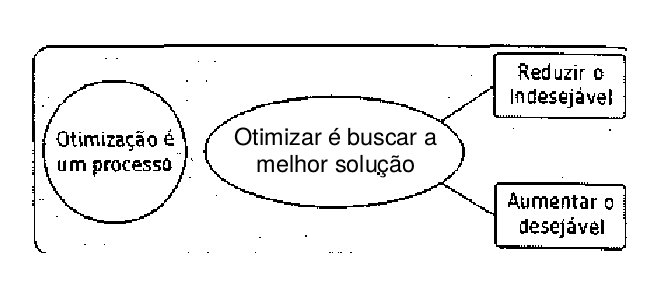
\includegraphics[width=.9\textwidth]{otimizacao/otimizacao}

\vfill
Fonte: BAZZO \& PEREIRA, 2006.
\end{frame}

\begin{frame}{Exemplos}
  \begin{itemize}
  \item geladeira
  \item panela de pressao
  \item rotas
  \item processos de construção
  \item matéria prima
  \item demanda e oferta (preços de venda)
  \end{itemize}
\end{frame}

\begin{frame}
  Métodos

  \begin{itemize}
  \item Evolução
  \item Intuição
  \item Tentativa
  \item Gráfico
  \item Analítico
  \end{itemize}
\end{frame}

\subsection{Métodos}

\begin{frame}
  \begin{block}{evolução}
    A otimização por evolução muitas vezes está relacionada com a
    evolução tecnológica. Ela acontece quando um sistema já existente
    é aperfeiçoado através de alterações e melhorias na sua concepção,
    processo de fabricação ou mesmo no aspecto estético. Com isso, ao
    longo do tempo, tem-se um sistema mais eficiente e moderno.
  \end{block}

\vfill
Fonte: BAZZO \& PEREIRA, 2006.
\end{frame}

\begin{frame}
    \begin{block}{intuição}
    O projeto em engenharia - que é um processo criativo - é altamente
dependente da arte. Na área técnica, a arte está relacionada, por exemplo, com
a habilidade para ter boas soluções ou para modelar sistemas - em forma
física ou matemática -, mesmo que não conheçamos uma justificativa com
base científica para explicar o problema.
  \end{block}

\vfill
Fonte: BAZZO \& PEREIRA, 2006.
\end{frame}

\begin{frame}
    \begin{block}{tentativa}
    O projeto, conforme já enfatizado, é um processo iterativo. E
    iniciado com um esboço preliminar da solução - que normalmente é
    pobre -- e, através de refinos e novas definições, chega-se a um
    resultado final melhor que a proposta inicial. Isso é normal num
    projeto, pois usualmente a primeira alternativa não é
    satisfatória, sendo necessárias novas tentativas para encontrar
    uma boa solução.
  \end{block}

\vfill
Fonte: BAZZO \& PEREIRA, 2006.
\end{frame}

\begin{frame}
  \begin{block}{gráfica}
    A técnica de otimização gráfica consiste, basicamente, na
utilização de esquemas ou desenhos de um sistema físico real na procura da
melhor solução para o problema em análise.
  \end{block}

\vfill
Fonte: BAZZO \& PEREIRA, 2006.
\end{frame}

\begin{frame}
  \begin{block}{analítica}
    Esta é a área mais recente da otimização, sendo baseada no
    desenvolvimento matemático.
  \end{block}

\vfill
Fonte: BAZZO \& PEREIRA, 2006.
\end{frame}

\begin{frame}
  \begin{block}{uma variável}
    O caso mais simples de otimização ocorre quando temos apenas uma
    variável envolvida. Podemos, então, representar o sistema a
    otimizar por uma função que contém uma variável independente x e
    uma variável dependente.  Uma expressão matemática para isso pode
    ser: y = f (x), onde x é a variável independente, que pode
    assumir, em princípio, qualquer valor, e y é a variável dependente
    de x, ou seja, dependendo do valor que x assumir, teremos um valor
    específico para y.
  \end{block}

\vfill
Fonte: BAZZO \& PEREIRA, 2006.
\end{frame}

\begin{frame}
    \begin{block}{uma variável}
    O processo de otimização, neste caso, resume-se a encontrar o
    valor limite de y, ou seja, o máximo valor de alguma quantidade
    desejável ou o mínimo valor de uma característica indesejável.
  \end{block}

\vfill
Fonte: BAZZO \& PEREIRA, 2006.
\end{frame}

\begin{frame}
  \begin{block}{duas ou mais variáveis}

  \end{block}

\vfill
Fonte: BAZZO \& PEREIRA, 2006.
\end{frame}

\begin{frame}

\end{frame}

\subsection[Curiosidade]{Curiosidade: Otimização matemática}

\begin{frame}{Curiosidade}
  \begin{block}{Atenção}
    Esta seção da aula não faz parte da matéria, e será explorada nas disciplinas dos próximos semestres.
  \end{block}
\end{frame}

\begin{frame}{Curiosidade}
A matemática aplicada nos proporciona diversos métodos para encontrar soluções ótimas para problemas práticos:

  \begin{enumerate}
  \item<2-> Otimização linear com restrições
  \item<3-> Otimização não-linear sem restrições
  \item<4-> Otimização não-linear com restrições
  \end{enumerate}
\end{frame}

\begin{frame}{Otimização linear com restrições}
  \begin{itemize}
  \item Programação linear (pesquisa operacional)
  \item Algoritmo SIMPLEX
  \item O espaço de soluções viáveis é um polígono
  \item O algoritmo resolve um sistema de inequações lineares
  \item A solução ótima está na fronteira do espaço de soluções
  \end{itemize}
\end{frame}

\begin{frame}{Otimização não-linear sem restrições}
  \begin{itemize}
  \item Cálculo Diferencial de funções (Cálculo I)
  \item Derivada da função: $\frac{d f}{d x}(x)$
  \item A solução ótima está onde a derivada se anula
  \end{itemize}
\end{frame}

\begin{frame}{Otimização não-linear sem restrições}
  \begin{itemize}
  \item Cálculo Diferencial vetorial (Cálculo II)
  \item Vetor gradiente: $\nabla f(x,y)$
  \item A solução ótima está onde o vetor gradiente se anula
  \end{itemize}
\end{frame}

\begin{frame}{Otimização não-linear com restrições}
  \begin{itemize}
  \item Cálculo Diferencial Vetorial (Cálculo II)
  \item Multiplicadores de Lagrange
  \item Resolver um sistema de equações não-lineares
  \item A solução ótima está na fronteira do espaço de soluções
  \end{itemize}
\end{frame}

\end{document}
